\subsection{Approximating $\pi$}
\label{approx-pi}

We demonstrate different sampling strategies through the well-known problem of estimating $\pi$ by approximating the area of a unit circle inscribed in a square. A comprehensive analysis including implementation details and extended theoretical background can be found at \href{https://nikogerman.github.io/Seminar/Notebooks/example1-estimating-pi.html}{\texttt{example1-estimating-pi.html}}. In the following, we discuss only the general setup and key results.

Since the unit circle has area $\pi$ and the enclosing square $[-1,1] \times [-1,1]$ has area 4, we obtain the estimator $\hat{\pi} = 4 \cdot \mathbb{P}(X^2 + Y^2 \leq 1)$ where $(X,Y)$ are sampled from the square.

\textbf{Sampling Methods Compared:} We compare uniform Monte Carlo sampling, importance sampling with $\mathcal{N}(0, \sigma^2 I_2)$ where $\sigma = 1/3$, quasi-Monte Carlo using Sobol sequences, and grid-based deterministic quadrature.

\begin{figure}[h]
    \centering
    \begin{subfigure}[b]{0.48\textwidth}
        \centering
        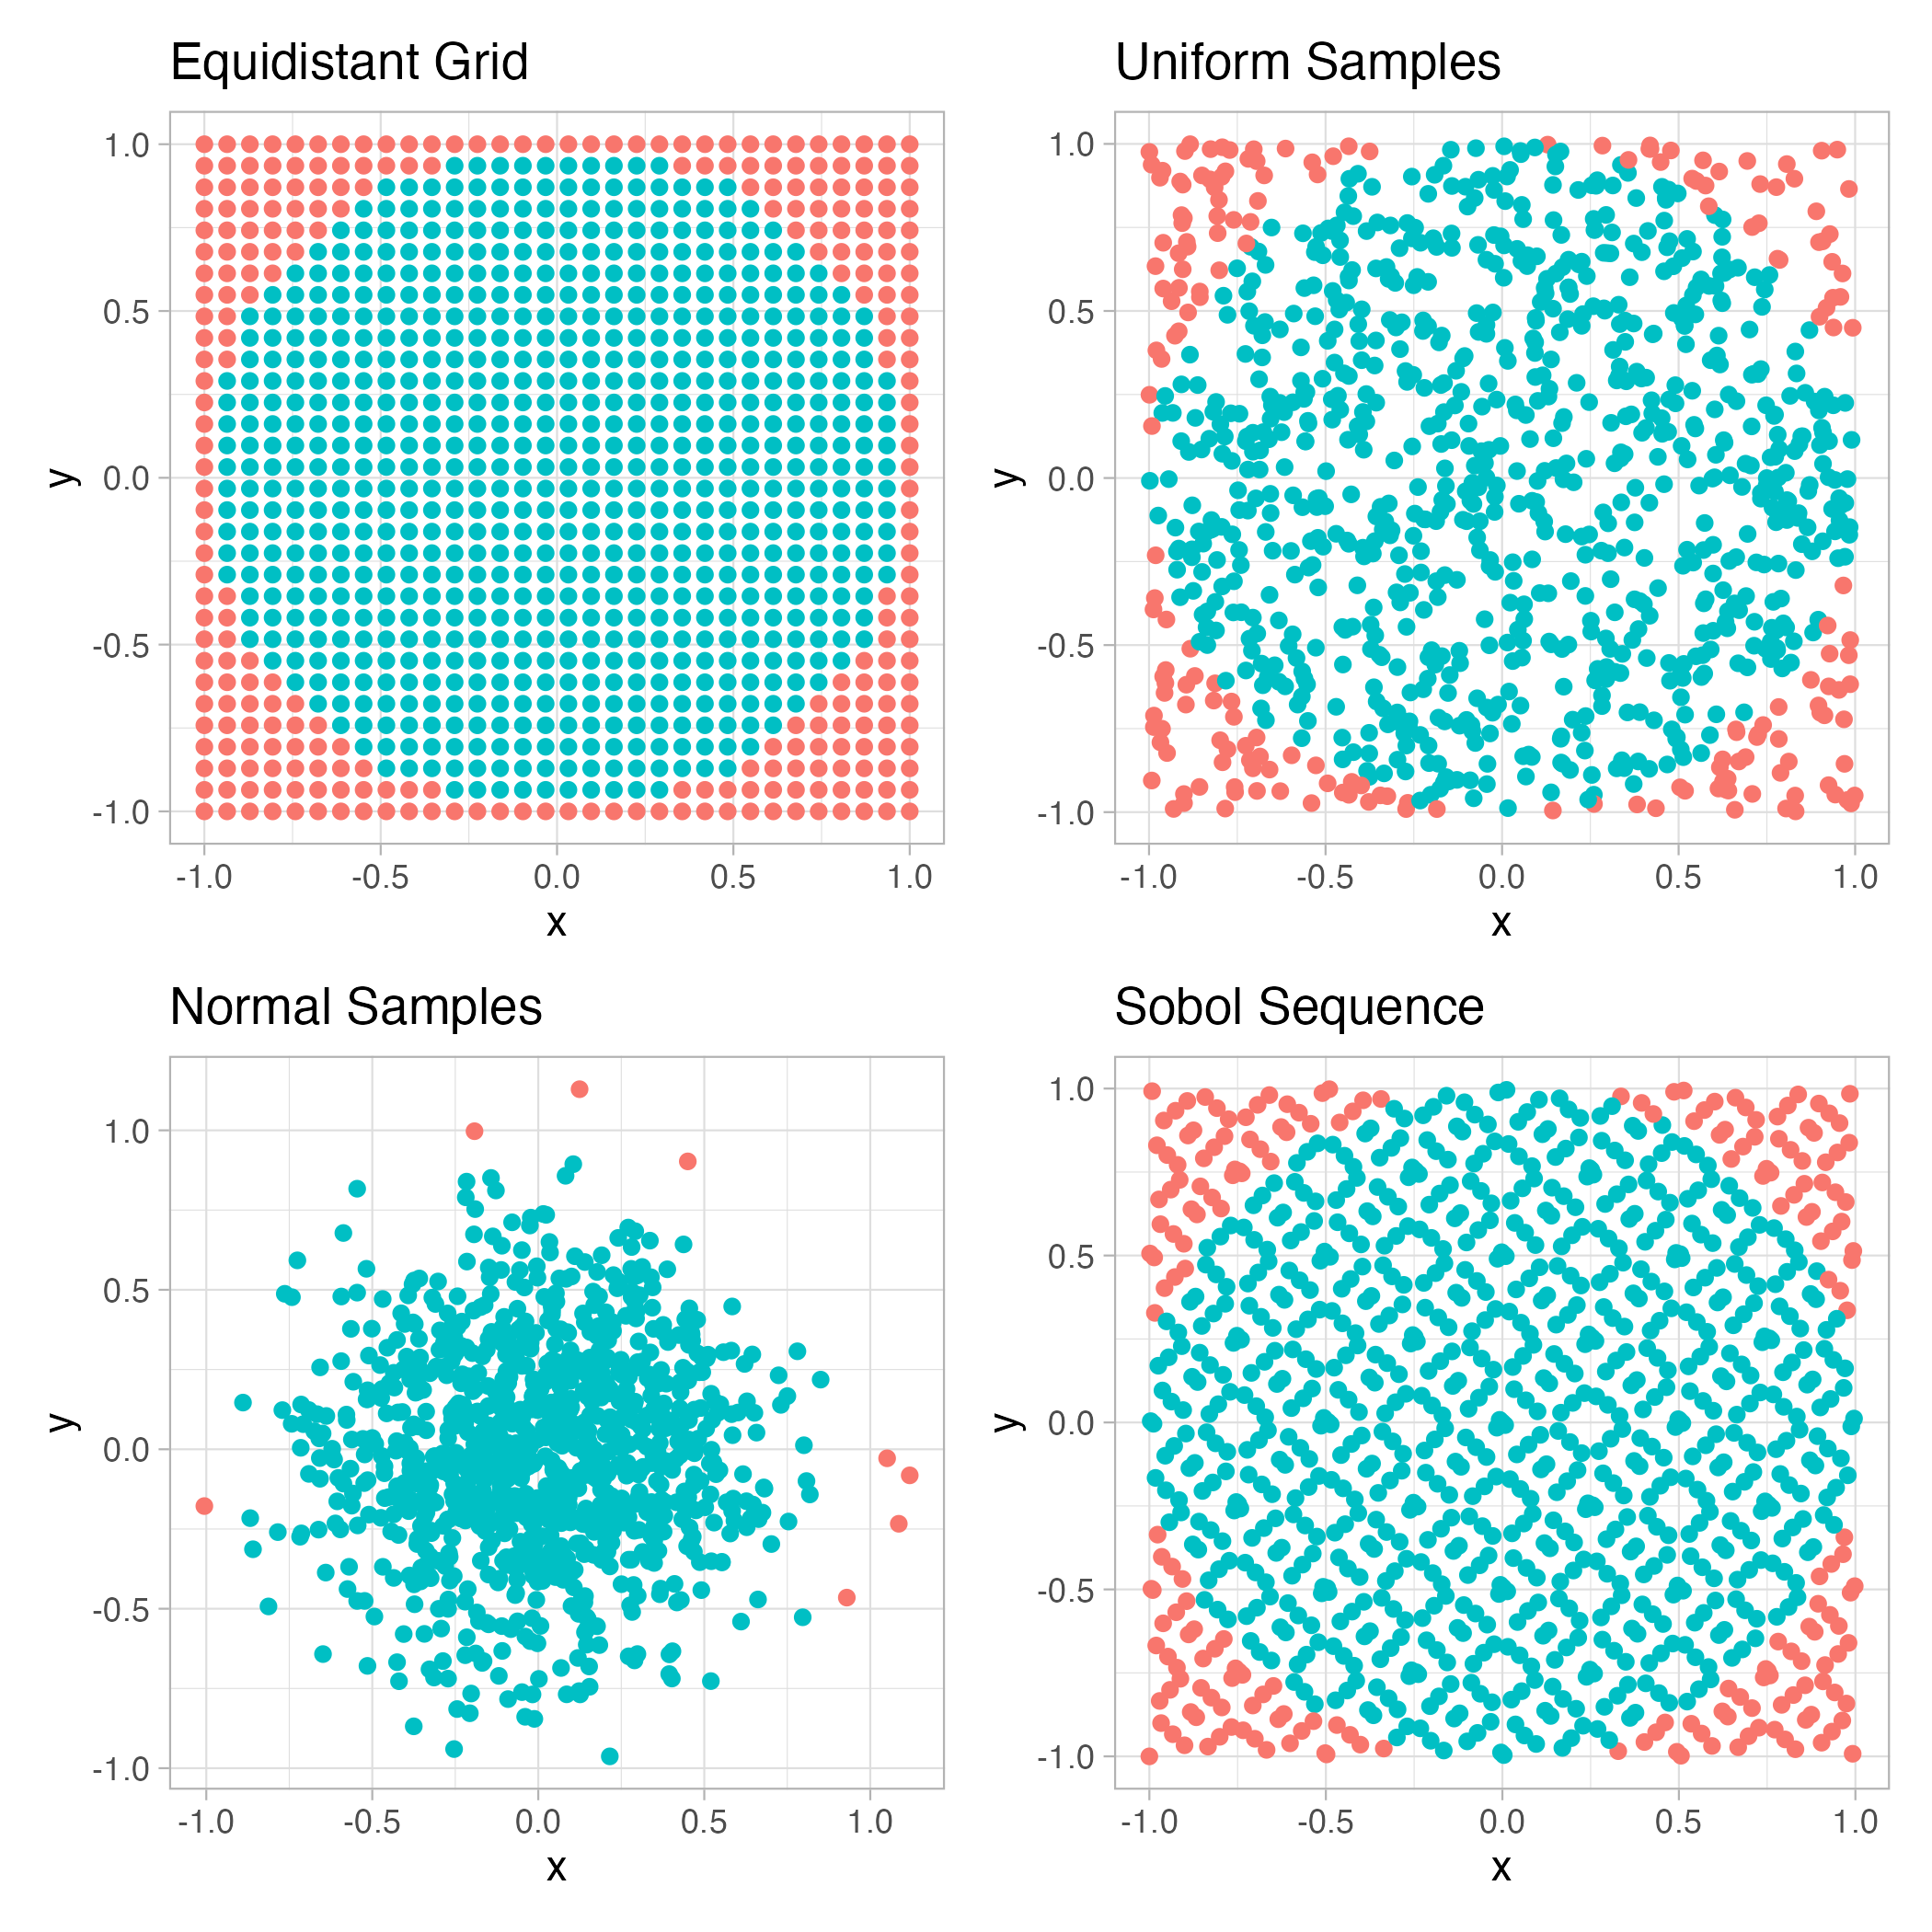
\includegraphics[width=\textwidth]{figures/ex1-samples.png}
        \caption{Visualization of the four sampling strategies, each with $2^{10} = 1024$ points colored by whether they fall inside the unit circle.}
        \label{fig:ex1-samples}
    \end{subfigure}
    \hfill
    \begin{subfigure}[b]{0.48\textwidth}
        \centering
        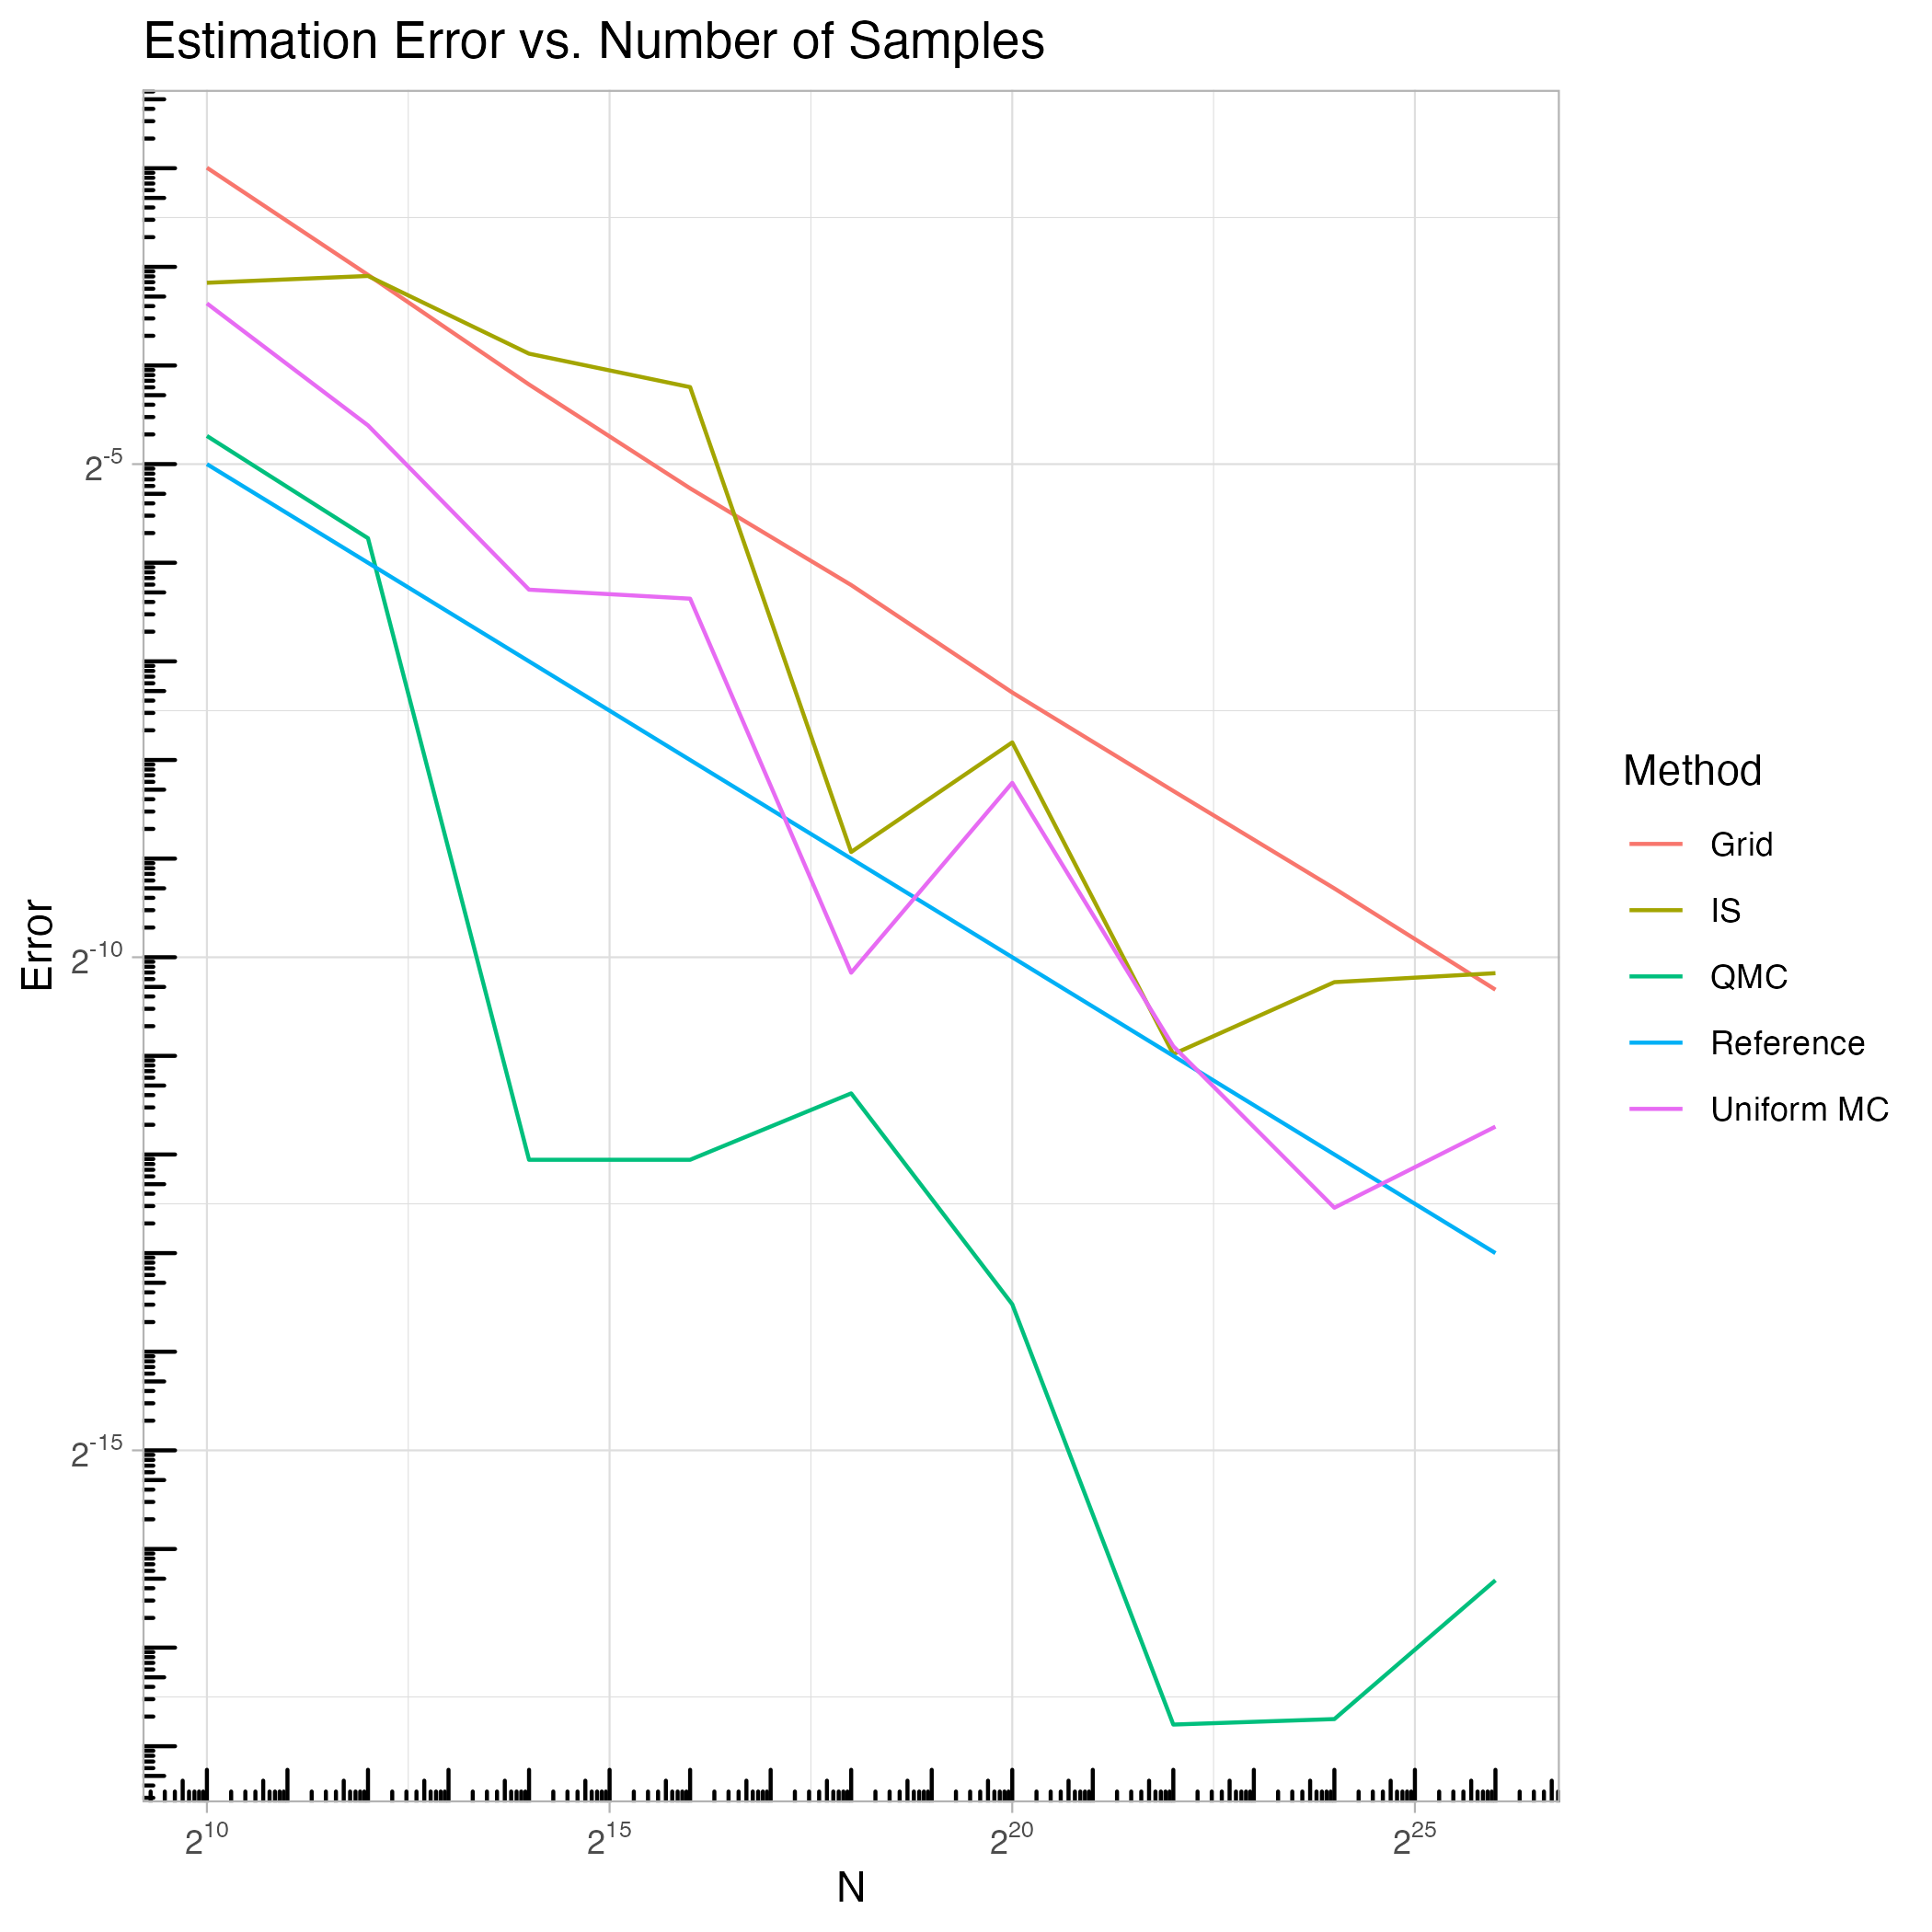
\includegraphics[width=\textwidth]{figures/ex1-estimation-error.png}
        \caption{Convergence comparison showing absolute error versus sample size. Sobol sequences demonstrate superior performance due to space-filling properties.}
        \label{fig:ex1-estimation-error}
    \end{subfigure}
    \caption{Comparison of sampling strategies for $\pi$ estimation. Generated using \href{https://github.com/NikoGerman/Seminar/blob/main/Notebooks/example1-estimating-pi.Rmd}{\texttt{example1-estimating-pi.Rmd}}.}
    \label{fig:pi-estimation-comparison}
\end{figure}

\textbf{Key Results:} Figure~\ref{fig:pi-estimation-comparison} shows that Sobol sequences demonstrate superior performance with consistently lower errors due to space-filling properties. Uniform Monte Carlo exhibits the expected $O(N^{-1/2})$ convergence, while the chosen importance sampling parameters provide no variance reduction for this problem.

\subsection{Probability of Rare Events}
\label{rare-events}

Estimating probabilities of rare events presents a fundamental challenge for standard Monte Carlo methods due to high variance and poor convergence. 
We demonstrate this challenge through a portfolio risk model where we estimate the probability of a remarkably high profit. In the following, we will discuss only the general setup and key results.
A comprehensive analysis of this problem, including theoretical background and implementation details, can be found at \href{https://nikogerman.github.io/Seminar/Notebooks/example2-rare-event.html}{\texttt{example2-rare-event.html}}. 

\textbf{Portfolio Setup:} Consider a portfolio with initially equally weighted assets, where each stock's log-return follows $Z_i \sim \mathcal{N}(\mu_i, \sigma_i^2)$ with parameters $\boldsymbol{\mu} = (-0.1, 0.2, -0.3, 0.1, 0)$ and $\boldsymbol{\sigma}^2 = (0.3, 0.3, 0.3, 0.2, 0.2)$. The portfolio value is $S = \sum_{i=1}^5 \exp(Z_i)$. Our objective is to estimate $\mathbb{P}(\bar{S} > 4)$, representing a 300\% profit.

\textbf{Methods Compared:} Standard Monte Carlo samples directly from the original distributions, while importance sampling uses shifted parameters $\tilde{\mu}_i = 1$ and $\tilde{\sigma}_i = 1$ to make the rare event more likely, then corrects using importance weights.

\textbf{Key Result:} For this rare event with probability $P \approx 2.3 \times 10^{-6}$, importance sampling achieves dramatically lower relative errors compared to standard Monte Carlo, enabling practical estimation of tail probabilities, as demonstrated in Figure \ref{fig:rare-events-analysis}.

\begin{figure}[h]
    \centering
    \begin{subfigure}[b]{0.48\textwidth}
        \centering
        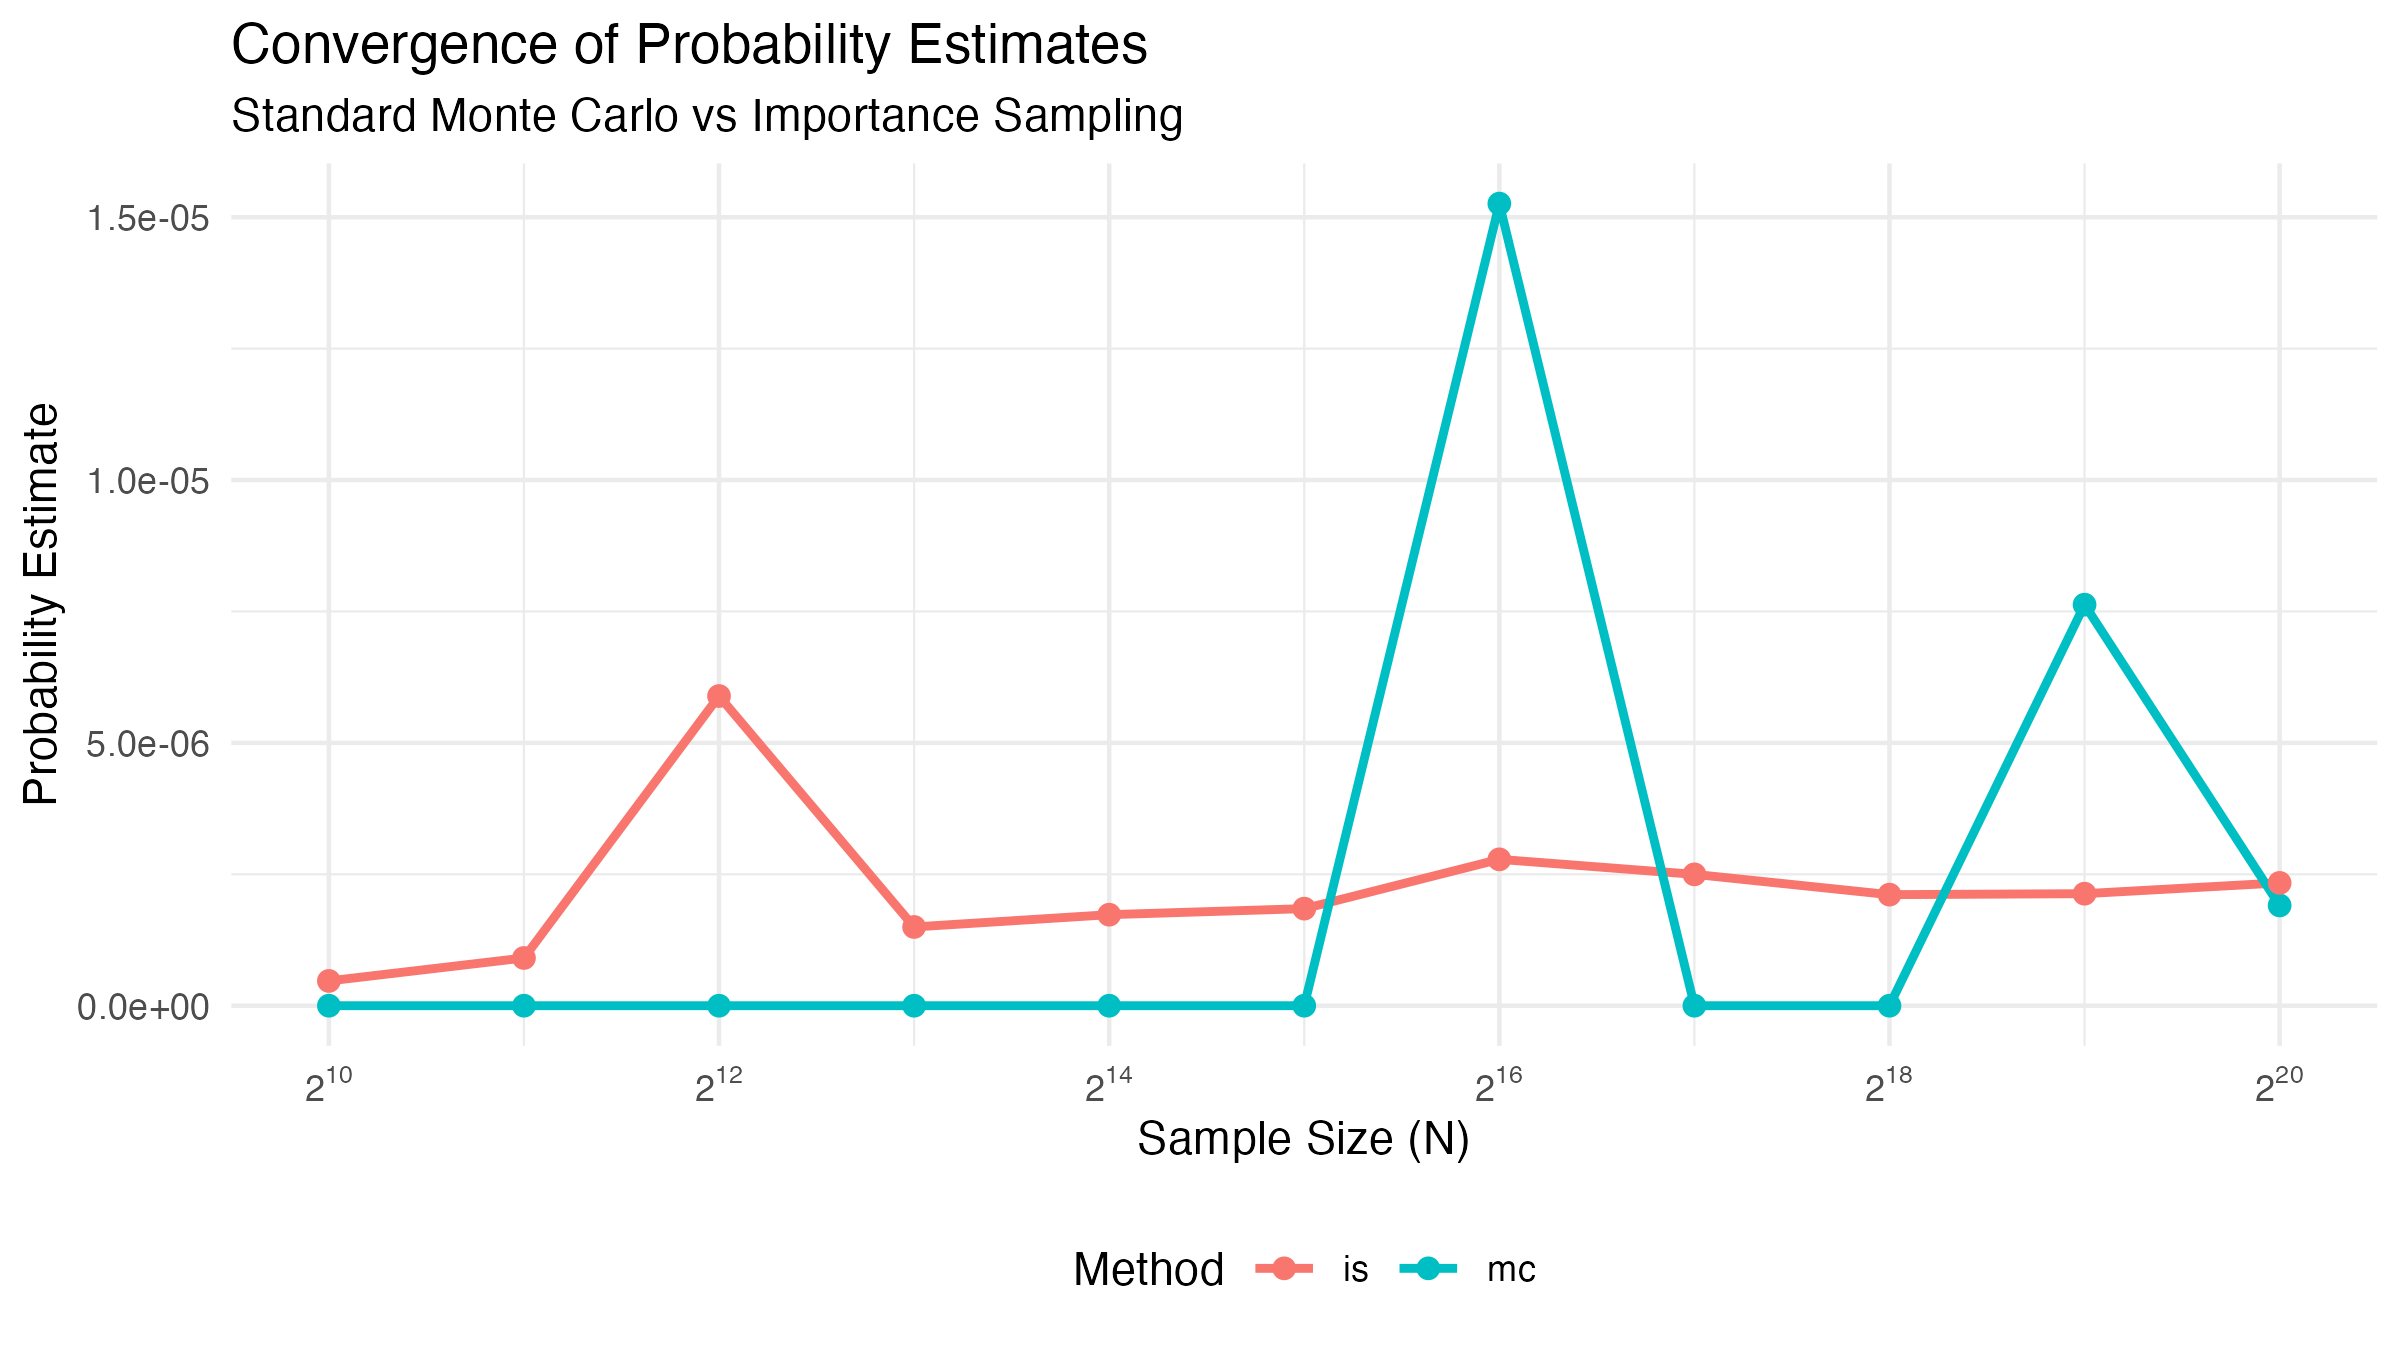
\includegraphics[width=\textwidth]{figures/ex2-estimates.png}
        \caption{Probability estimates versus sample size showing the superior convergence of importance sampling.}
        \label{fig:rare-events-estimates}
    \end{subfigure}
    \hfill
    \begin{subfigure}[b]{0.48\textwidth}
        \centering
        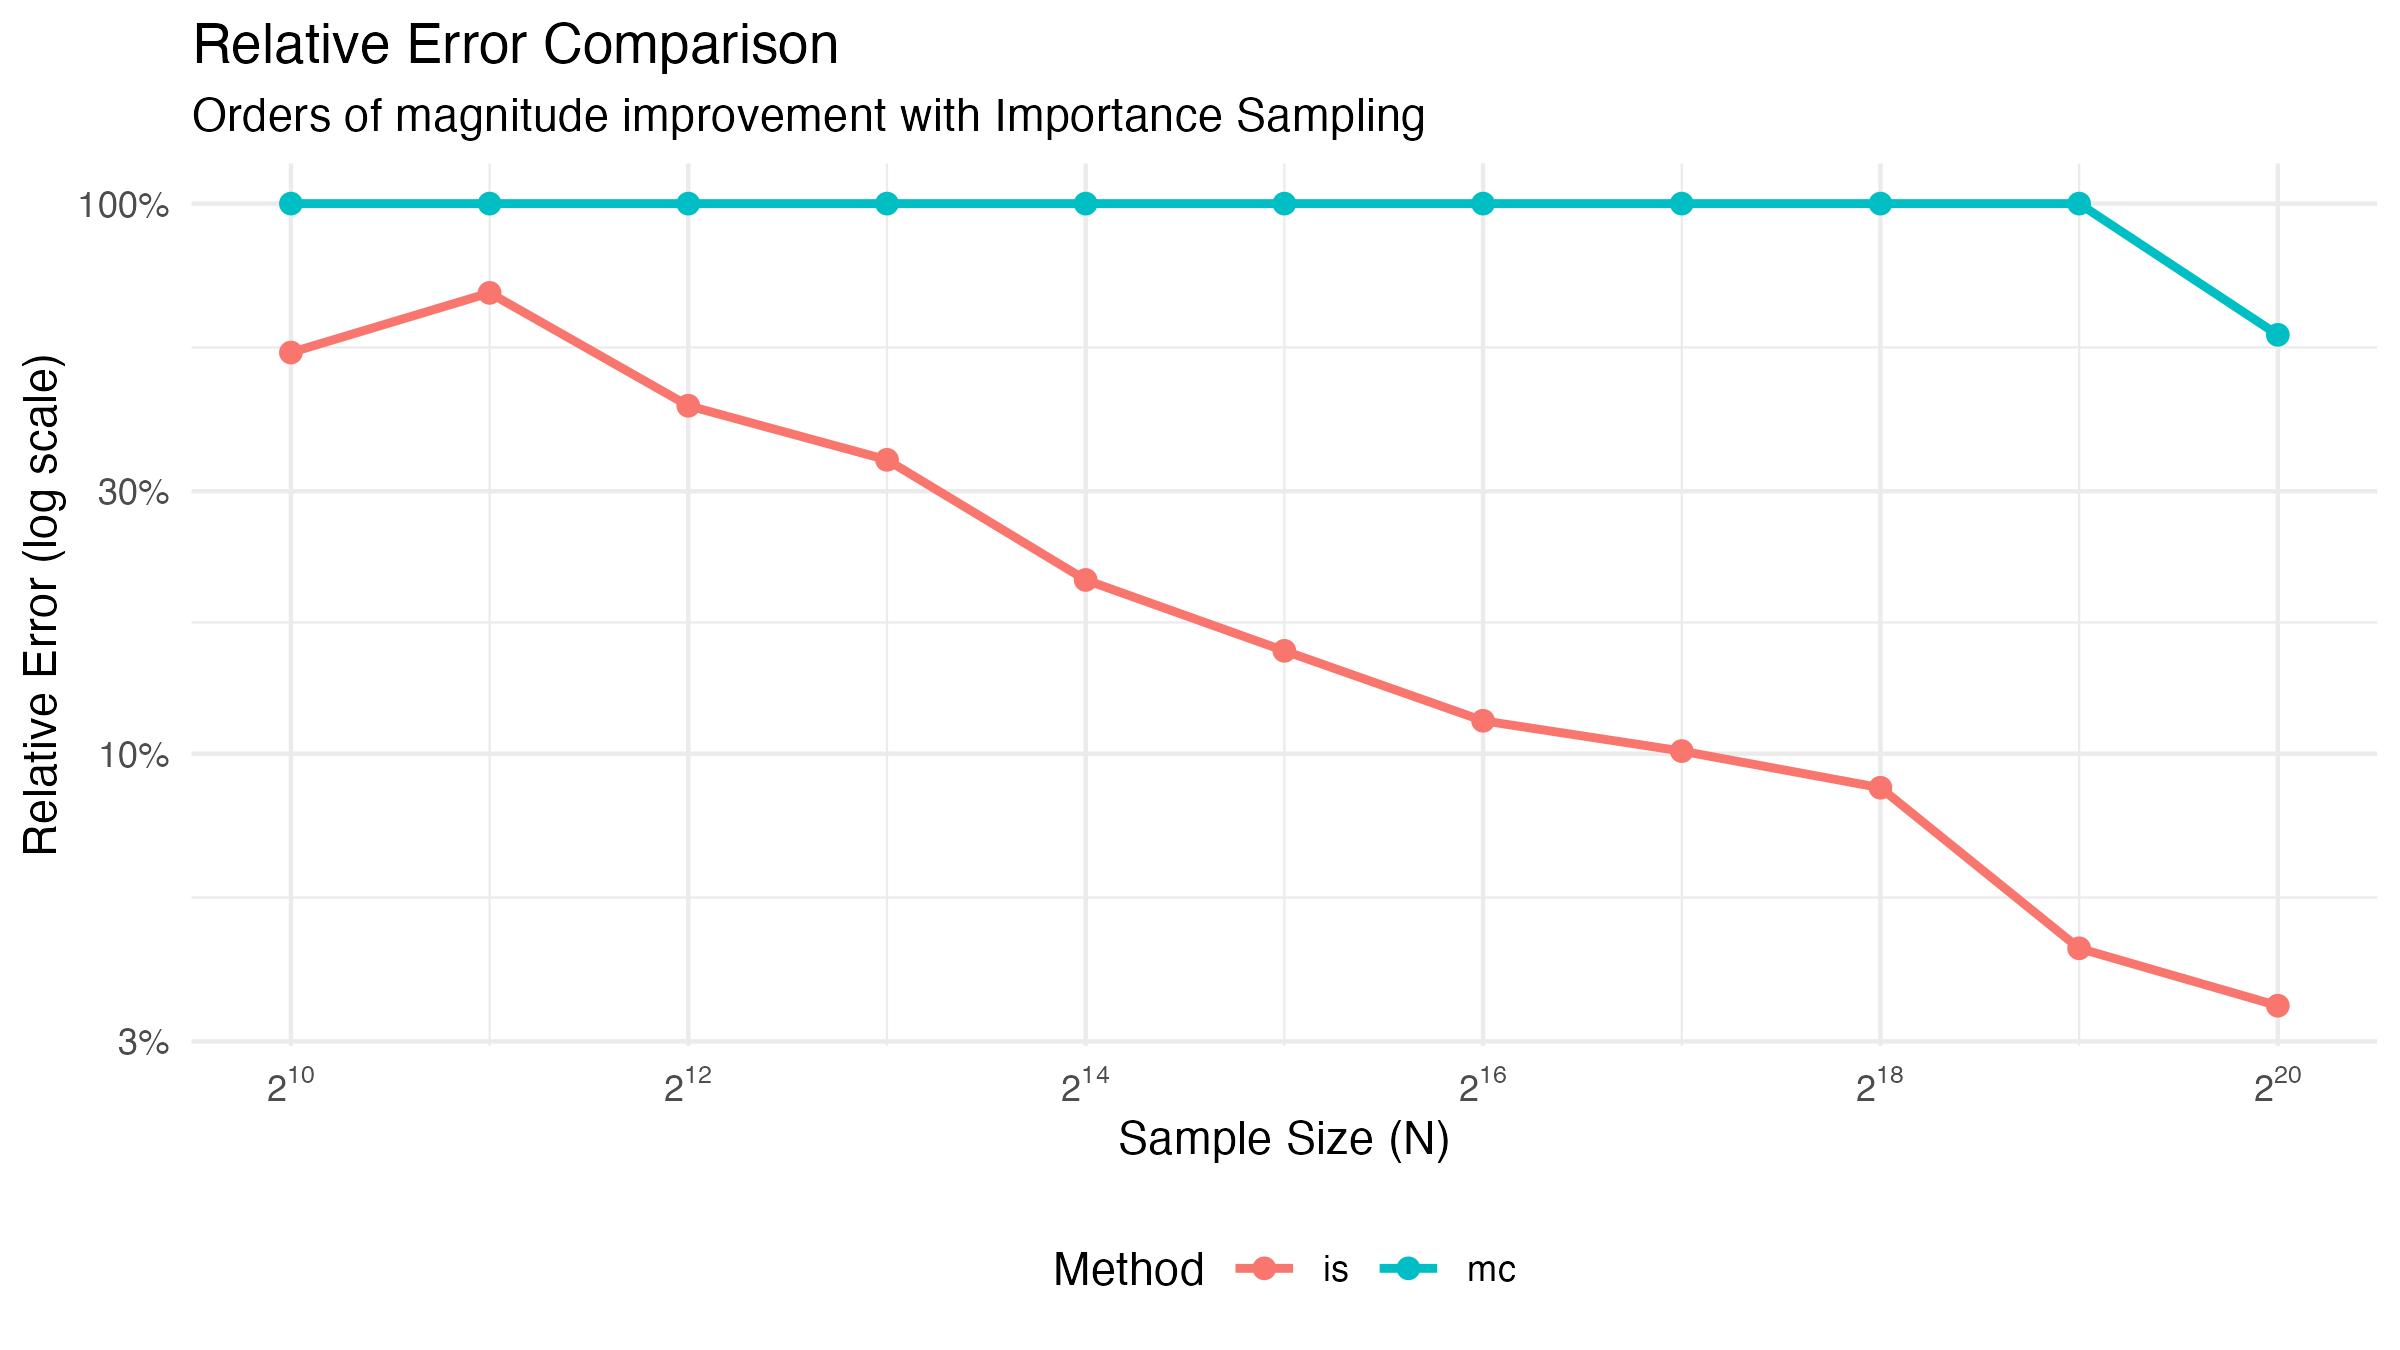
\includegraphics[width=\textwidth]{figures/ex2-rel-errors.png}
        \caption{Relative error comparison demonstrating orders of magnitude improvement with importance sampling.}
        \label{fig:rare-events-relative-errors}
    \end{subfigure}
    \caption{Comparison of standard Monte Carlo versus importance sampling for rare event estimation. Generated using \href{https://github.com/NikoGerman/Seminar/blob/main/Notebooks/example2-rare-event.Rmd}{\texttt{example2-rare-event.Rmd}}.}
    \label{fig:rare-events-analysis}
\end{figure}

This example illustrates why importance sampling is essential for applications requiring accurate tail probability estimation.